\chapter{TINJAUAN PUSTAKA}

% Ubah konten-konten berikut sesuai dengan isi dari tinjauan pustaka
\section{Hasil Penelitian Terdahulu}
% \section{Kendali mobil robot menggunakan isyarat tangan berbasis arduino}
Pada November 2020, Jati Widyo Leksono, Agung Samudra, Nanndo Yannuansa, dan Ahmad Fauzi membuat jurnal mengenai sistem kendali \textit{mobile robot} menggunakan isyarat tangan. Dalam penelitian ini akan dilakukan pengembangan \textit{mobile robot} yang mampu berjalan sesuai dengan isyarat tangan atau gestur tangan yang diberikan oleh user. Pada telapak tangan user nantinya akan ditempelkan suatu sensor yang mampu membaca pergerakan telapak tangan menurun, naik, kiri, kanan, dan mendatar. Dari pembacaan sensor tersebut data akan dikirimkan menuju \textit{receiver} yang terdapat pada robot secara \textit{wireless} \parencite{JurnalElectroLuecat}.

\section{Teori Dasar}

\subsection{Mobile Robot}
Robot merupakan suatu perangkat otomatis yang dapat menjalankan suatu tugas yang berasal dari manusia \parencite{Desainrobot}.
Mobile Robot merupaka salah satu jenis robot yang dapat berpindah posisi dari satu titik ke tiitk yang lain. Perpindahan robot ini dapat dimungkinkan dengan adanya suatu aktuator yang memungkinkan untuk menggerakkan keseluruhan badan robot. Salah satu contoh dari mobile robot adalah robot beroda yang terdiri dari dua buah roda yang berpasangan pada kanan dan kiri robot serta digerakkan memutar oleh aktuator. Pergerakan robot beroda akan diatur oleh arah serta kecepatan putaran robot. Pada saat arah serta kecepatan putaran roda sama maka robot akan bergerak lurus, namun jika arah atau kecepatan putaran roda ada yang berbeda pada satu sisi roda maka akan membuat robot berbelok \parencite{mobilerobot}. \textit{Mobile Robot} dapat dikendalikan jika terdapat \textit{remote control} yang menghubungkan pengguna dengan robot. \textit{Remote control} ketika digunakan oleg pengguna akan mengirimkan suatu sinyal navigasi kepada mikrokontroller yang terdapat pada robot. Mikrokontroller ini yang nantinya akan menerjemahkan sinyal yang diterima dan meneruskannya menjadi kontrol untuk menggerakkan robot.


\subsection{Estimasi Pose Tangan}
\begin{figure}[!h]
  \centering
	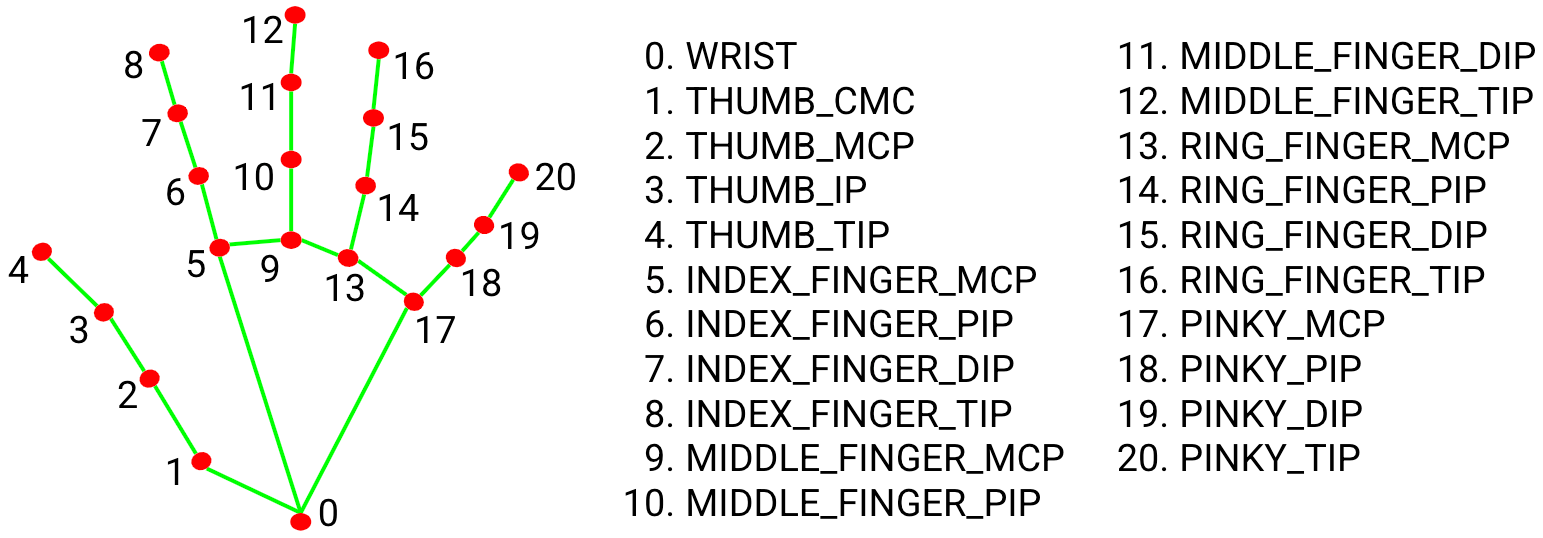
\includegraphics[width=0.7\linewidth]{../Gambar/hand_landmarks.png}
	\caption{Dua puluh satu titik \textit{keypoint} pada tangan \parencite{mediapipe}}
	\label{fig:tangan}
\end{figure}
Pengenalan gestur atau pose tangan merupakan topik yang menarik dalam ilmu komputer dan teknologi yang betujuan untuk komunikasi antara manusia dengan komputer menggunakan gestur tanpa menyentuhnya secara langsung. Saat ini banyak \textit{framework} atau \textit{library} pembelajaran mesin untuk mengenali gerakan tangan, salah satu yaitu \textit{Mediapipe}. \textit{Mediapipe} merupakan suatu framework yang dirancang oleh Google untuk menghasilkan audio atau video dari membangun \textit{pipelines} untuk mengolah data persepsi. Dengan bantuan dari \textit{Mediapipe} tangan yang terdapat pada citra akan dapat dideteksi dengan mendeteksi dua puluh satu titik pada tangan yang ditunjukkan oleh Gambar \ref*{fig:tangan}. Proses pertama yaitu akan mendeteksi telapak tangan atau disebut \textit{palm detection} agar program dapat mendeteksi keberadaan tangan. Selanjutnya yaitu mendeteksi dua puluh titik \textit{keypoint} dalam tangan yang sudah terdeteksi \parencite{UniversitasDinamika}. 


\subsection{\textit{Convolutional Neural Network} (CNN)}
\begin{figure}[!h]
  \centering
  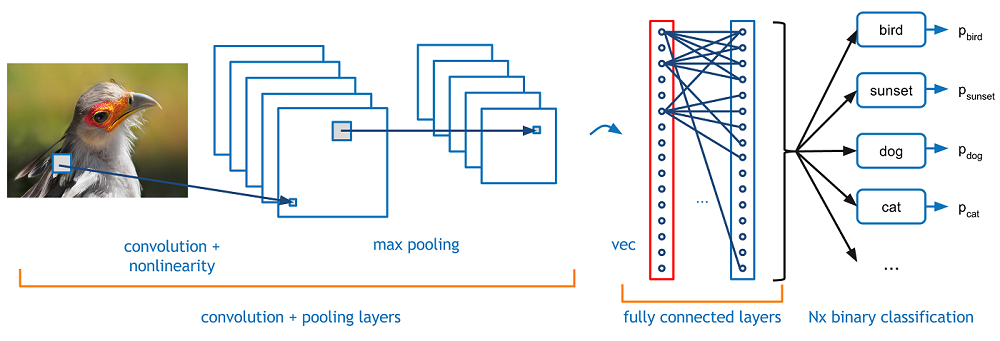
\includegraphics[width=1\linewidth]{../Gambar/cnn.png}
  \caption{Arsitektur CNN \parencite{adit}}
  \label{fig:cnn}
\end{figure}
CNN merupakan salah satu dari \textit{neural network} yang digunakan untuk memproses data berupa grid. Salah satu contoh dari data grid adalah citra. Citra dianggap sebagai grid karena berbentuk piksel dua dimensi. CNN dianggap sebagai salah satu solusi untuk permasalahan pada bidang \textit{Computer Vision} untuk mendeteksi dan mengenali sebuah image \parencite{CNN}. Secara nama CNN menunjukkan bahwa operasi matematika yang akan digunakan yaitu konvolusi dengan cara mengkalikan data dua dimensi dengan kernel. Pada CNN akan memiliki 3 lapisan utama seperti pada Gambar \ref*{fig:cnn} yaitu :
\begin{enumerate}
  \item \textit{Convolutional Layer} \par
  Layer ini merupakan inti dari CNN karena pada layer ini akan dilakukannya operasi konvolusi. Operasi konvolusi pada layer ini akan dilakukan antara input data dengan \textit{filter} atau \textit{kernel}. \textit{Filter} akan melintasi input data dan akan melakukan operasi "dot" antara input data dengan nilai dari \textit{filter} sehingga akan menghasilkan \textit{feature map} \parencite{LinaQ}.
  
  \item \textit{Pooling Layer} \par
  Layer ini digunakan untuk melakukan \textit{downsampling} yang berguna untuk mengurangi dimensi dan jumlah parameter. Terdapat dua jenis \textit{pooling} yang sering digunakan yaitu \textit{max pooling} dan  \textit{average pooling}. \textit{Max pooling} adalah mengambil citra maksimum yang dicakup oleh kernel, sedangkan pada \textit{average pooling} adalah mengambil nilai rata-rata dari citra yang dicakup kernel.
  Namun tidak hanya itu \textit{pooling layer} juga digunakan untuk mengekstraksi fitur dominan \parencite{Bukusakti}. 

  \item \textit{Fully Connected Layer} \par
  Layer ini digunakan untuk melakukan transformasi pada dimensi data agar dapat diklasifikasikan secara liner.
  Hasil dari \textit{pooling layer} masih berbentuk \textit{multidimensional array}, maka dari itu pada \textit{fully connected layer} akan dilakukan \textit{reshape} input dari \textit{multidimensional array} menjadi vector. Setiap \textit{neuron} pada \textit{convolutional layer} akan ditransformasikan menjadi data satu dimensi sebelum dapat dimasukkan dalam sebuah \textit{fully connected layer} \parencite{JurnalTeknikITS}.
\end{enumerate} 

